\chapter{3D目标位姿估计算法}
\label{chap:pose}
本章提出了一种3D目标位姿估计算法3D-MRAI(3D Mask R-CNN \& A4PCS-ICP),该算法根据所提供目标的CAD模型,可以在RGB-D图中检测出目标,并给出目标的位姿。3D-ODPE算法主要基于第~\ref{chap:detector}~章中基于RGB-D图的目标检测算法3D Faster R-CNN/3D Mask R-CNN,以及第~\ref{chap:matcher}~章中的点云匹配算法A4PCS-ICP,通过将这两个算法结合,分两步计算出RGB-D图中目标的位姿。为了评价3D-MRAI算法的性能,本章还设计了相关实验,并与同类算法做了比较。

\section{3D-MRAI框架设计}
3D-MRAI主要解决三维空间中的目标检测和位姿估计问题,根据RGB-D图像,给出图像中目标的种类和其在三维空间中的位姿,区别与常见的在2D图像中的目标检测(如第~\ref{chap:detector}~章中的算法)给出的是目标的种类和其在图像坐标中的bounding box或者mask。给出目标在三维空间中的位姿的意义十分巨大,尤其在机器人领域中,图像层面的结果往往难以满足要求,但难度也很大。

一些给出3D目标位姿的传统算法,如3DMatch\cite{zeng20163dmatch},3DMatch通过匹配局部几何特征来计算目标的位姿,缺点是对采集的3d数据质量要求很高,往往需要使用激光采集,因此整个识别过程的时间很久;通过SIFT描述子来匹配目标位姿\cite{dias2015sift}也是一种方法,但其对纹理较少的物体往往难以匹配,效果很差;另外如LINEMOD\cite{hinterstoisser2012gradient}和MOPED\cite{collet2011moped}这些位姿估计框架,在某些情况下如目标在平整的桌面上并且光照条件较好的情况下才能取得满意的效果。因此,急需一种鲁棒性较强,精度较高,计算时间较短的3D目标位姿估计算法。

3D-MRAI的框架如图\ref{fig:detect-pose}所示,
\begin{figure}[ht]
  \centering
  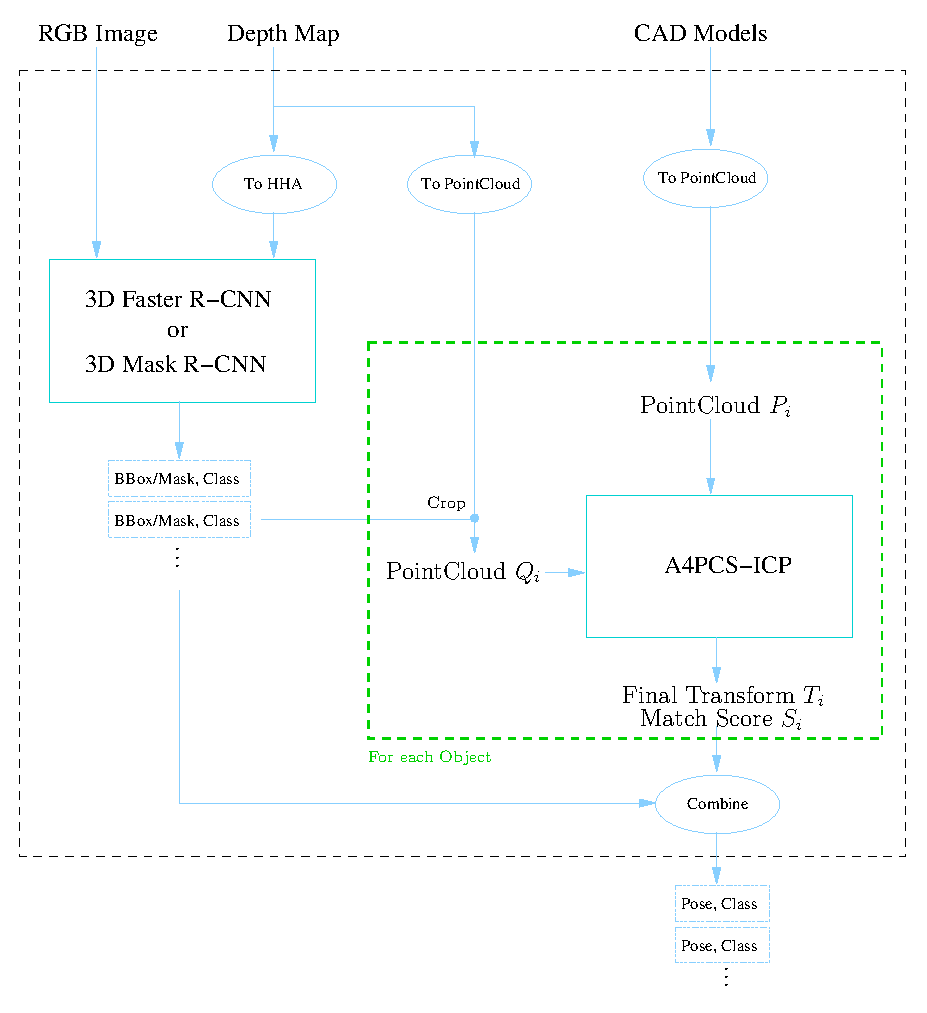
\includegraphics[width=12cm]{detect-pose}
  \caption{3D-MRAI算法框架}
  \label{fig:detect-pose}
\end{figure}
从图\ref{fig:detect-pose}可以看出算法的输入是RGB图像、深度图,以及目标物体的CAD模型,输出是图像中检测到的目标的位姿。3D-MRAI的核心部分是3D Faster/Mask R-CNN和A4PCS-ICP算法,3D Faster/Mask R-CNN以及在第~\ref{chap:detector}~章详细介绍过,A4PCS-ICP也在第~\ref{chap:matcher}~章详细介绍过了。因此,3D-MRAI估计目标的位姿流程上也是分为两步(two-stage):
\begin{itemize}
\item {\kai 目标检测}:利用3D Faster/Mask R-CNN检测目标,得到目标BBox或者Mask
\item {\kai 点云匹配}:将CAD模型与目标检测对应的点云进行匹配,得到目标位姿
\end{itemize}

\section{3D-MRAI具体实现}
对与3D-MRAI输入的RGB图像和深度图,可以由对偶RGB-D获得,具体见第~\ref{chap:rgbd}~章。目标物体的CAD模型也容易获得,对于工厂中的工件,往往是有其CAD模型的,对于一般物体,可以通过3D扫描仪重构出来,当然也可以使用本文设计的对偶RGB-D相机采集重构出来。

获得目标物体的CAD模型后,为了方便后续需处理,我们需要将其转换为点云。具体如何转换的话,基本思想是参考Uniform Sampling算法,Uniform Sampling算法的核心思想是以3D栅格中所有点的质心代替这些点,从而达到降采样。类似地,对于CAD模型也建立3D栅格,但由于无法获得3D栅格总所有点,因此判断CAD模型是否穿过3D栅格,如果穿过3D栅格,则在该3D栅格中心出增加一个点。显然3D栅格的边长越大,转换后的点云数量越小,精度越低,考虑到所使用相机生成点云的精度,因使CAD模型转换后的点云的精度与相机采集的点云的精度近似,实际取3D栅格边长为1mm,一个实际工件的CAD模型和以1mm为边长进行采样转换后的模型点云如图~\ref{fig:model-pc}~所示。
\begin{figure}[ht]
  \centering
  \subfloat[原CAD模型]{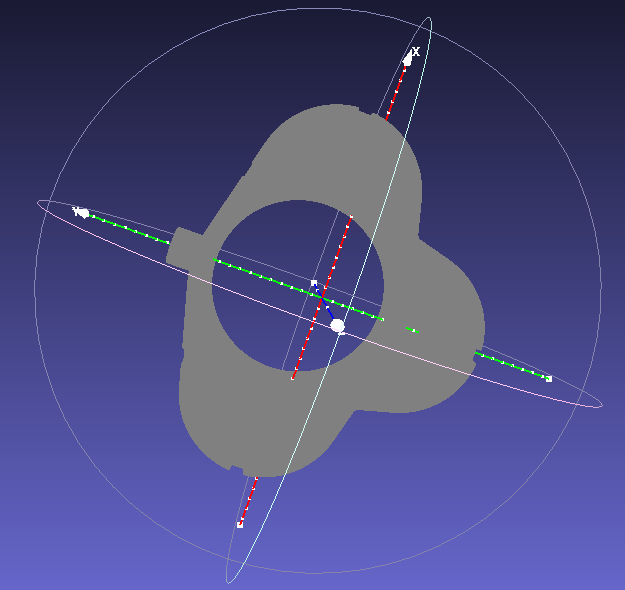
\includegraphics[width=7cm]{object-model}}
  \hskip1cm
  \subfloat[转换后点云]{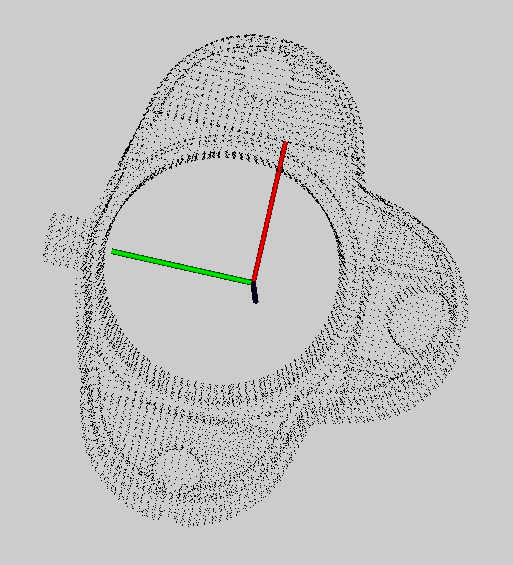
\includegraphics[width=6cm]{object-pointcloud}}
  \label{fig:model-pc}
  \caption{CAD模型和转换后的点云}
\end{figure}
此外,还需要将深度图转换为点云,这一步则相对简单,只要通过深度摄像头的内参矩阵反投影到三维空间即可,详细见第~\ref{chap:rgbd}~章。

对于3D Faster/Mask R-CNN的输入,还需要将深度图转换为HHA,具体见~\ref{sec:hha}~小节。3D Faster/Mask R-CNN模块的实现,由于一个深度神经网络,只要训练好后将网络模型导出成Tensorflow的pb文件,然后此处导入该网络模型,给定输入,网络输出便是图片中目标的BBox/Mask和Class。

得到目标物体的BBox/Mask后,需要从深度图对应的点云中抠出目标点云,由于深度图转换的点云是有序的,因此BBox/Mask在深度图中的索引坐标与深度图转换的点云的索引坐标是一致的,只要将点云中对应的点提取出来就行,并滤去无效的点然后适当降采样即可,尽管滤波和降采样之后的目标点云是无序的,但后续匹配算法并不需要输入点云有序,而且降采样后点云数量减少,将会减少后续匹配算法的时间。

裁剪得到目标物体的点云$Q_i$后,找出对应物体的CAD模型转换的点云$P_i$,将$P_i$和$Q_i$输入到A4PCS-ICP模型,即可得到CAD模型到目标点云之间的刚体变换$T_i$,由于CAD模型坐标系与相机坐标系重叠,因此将矩阵$T$转换为$X,Y,Z,r,p,y$就是目标点云在相机坐标系下的位姿Pose,最后将所有匹配得到的结果与目标检测的结果组合,并滤去匹配或检测分数较低的结果。详细的算法流程如算法\ref{alg:3d-mrai}所示。
\begin{algorithm}
  \caption{3D-MRAI算法}
  \label{alg:3d-mrai}
  \KwIn{RGB Image $I$, Depth Map $D$, CAD Models $M$}
  \KwOut{Set of Pose and Class $Res$}
  $Res\leftarrow \varnothing$\;
  $P\leftarrow \varnothing$\;
  \ForAll {$M_i\in M$} {
    $P\leftarrow \left\{P, CAD2PointCloud(M_i)\right\}$\;
  }
  $H = Depth2HHA(D)$\;
  $Q = Depth2PointCloud(D)$\;
  $Mask, Class \leftarrow 3DMASKRCNN(I, H)$\tcp*{Same with $3DFASTERRCNN$}
  \ForAll {$m_i\in Mask, c_i\in Class$} {
    $Q_i \leftarrow Crop(Q, m_i)$\;
    $P_i \leftarrow P(c_i)$\;
    $T_i,S_i\leftarrow A4PCSICP(P_i, Q_i)$\;
    \If {$S_i > S_{min}$} {
      $Res\leftarrow \left\{Res, \left[T_i, c_i\right]\right\}$\;
    }
  }
  \Return $Res$
\end{algorithm}

\section{3D目标位姿估计实验}
为了评价所提出的3D-MRAI的性能,设计了3D目标位姿估计的实验,并与文献\cite{hinterstoisser2012model}所提出的基于LINEMOD算法的3D目标位姿估计框架相比。
\subsection{数据集}
实验所使用的数据集是workpiece数据集,在第\ref{sec:dataset}小节中已经部分介绍过了,该数据集是在实验室采集的三类物体,第~\ref{chap:detector}~章中实验所用workpiece数据集中的ground truth是物体的种类、BBox和Mask,workpiece数据集中测试集中的图片的ground truth除了物体的种类、BBox和Mask,还有物体的位姿,物体的位姿是通过在物体旁固定标定板采集的。具体方法是,通过固定标定板在目标物体旁,我们可以记录标定板到目标的刚体变换关系$T_1$,然后我们通过彩色摄像头可以检测出标定板的位姿$T_2$,则物体的位姿可以通过下式得到
\begin{equation}
  T = T_2T_1
\end{equation}

\subsection{实验内容}
为了有效的评价3D-MRAI算法,我们先定义一个合适的评价指标{\kai 姿态误差}:
\begin{equation}
  m = {\underset{\mathbf{x}\in M}{avg}} \; {\parallel (R\mathbf{x}+t) - (\tilde{R}\mathbf{x}+\tilde{t})\parallel}
\end{equation}
其中$M$表示算法运行结果得到的物体种类对应的CAD模型转换得到的点云,$R$和$t$分别表示从ground truth物体位姿分解得到的旋转变换和平移变换,$\tilde{R}$和$\tilde{t}$分别表示从算法运行结果得到的物体位姿分解得到的旋转变换和平移变换。显然,如果算法运行结果和ground truth越接近,所定义的姿态误差就越小。对于一些对称的物体(如圆柱体的被子),显然不同角度下相机看到的目标物体可能近似,会造成算法运行的结果正确的情况下与ground truth相差很大,造成姿态误差很大,与我们所定义的评价指标的宗旨相违背。因此,针对一些对称的物体,重新定义姿态误差为
\begin{equation}
  m = {\avg_{\mathbf{x}_1\in M}} \; {\min_{\mathbf{x}_2\in M}} \; \norm{(R\mathbf{x}_1+t) - (\tilde{R}\mathbf{x}_2+t)}
\end{equation}
此外,如果$k_md>m$,我们就认为目标物体准确检测到了,并且估计的位姿正确,其中$d$是目标物体对应模型的直径,$k_m$是系数。因此,还可以定义一个正确检测目标并正确估计目标位姿的准确率。

实验在workpiece数据集的测试集上分别运行了3D-MRAI和文献\cite{hinterstoisser2012model}中的基于LINEMOD算法的检测框架,运行实验的计算机有两块Intel(R) Xeon(R) E5-2683 v3(2.00GHz)的CPU,4块TITAN X GPU,由于3D-MRAI有深度神经网络所以使用了一块GPU和一块CPU,Hinterstorisser等人的算法不需要GPU,只使用了一块CPU。

\subsection{实验结果}
@TODO: exp detect results figures
分别统计3D-MRAI和LINEMOD在测试集上的运行结果,变化系数$k_m$统计算法的准确率如表\ref{tab:mrai}所示。
\begin{table}[ht]
  \centering
  \begin{tabular}{ccccccc}
    \toprule
    $k_m[\%]$&5&7&9&11&13&15\\
    \midrule
    Hinterstorisser et al.&75.63& 83.84& 89.13& 93.48& 96.83&98.12\\
    \bf{3D-MRAI}&95.12& 97.35& 98.10& 98.69& 99.22& 100.00\\
    \bottomrule
  \end{tabular}
  \caption{3D-MRAI和Hinterstorisser等人的算法准确率}
  \label{tab:mrai}
\end{table}
表中$k_m$从$5\%$变化到$15\%$,表示物体直径的占比,$k_m$越大,允许的姿态误差就越大,因此准确率就越高。实际实验时,发现$k_m\approx 10\%$时基本上肉眼可以看出匹配的姿态误差。将表\ref{tab:mrai}绘制成图如\ref{fig:mrai}所示,从图中可以发现本文所提出的3D-MRAI算法的准确率大大超过了Hinterstorisser等人的算法,在$k_m=13\%$是3D-MRAI算法的准确率已经接近$100\%$了,以肉眼可以看出匹配的姿态误差$k_m=9\%$为标准时3D-MRAI算法的准确达到了$98.10\%$,比Hinterstorisser等人提出的算法高了大约$9$个百分点。
\begin{figure}[ht]
  \centering
  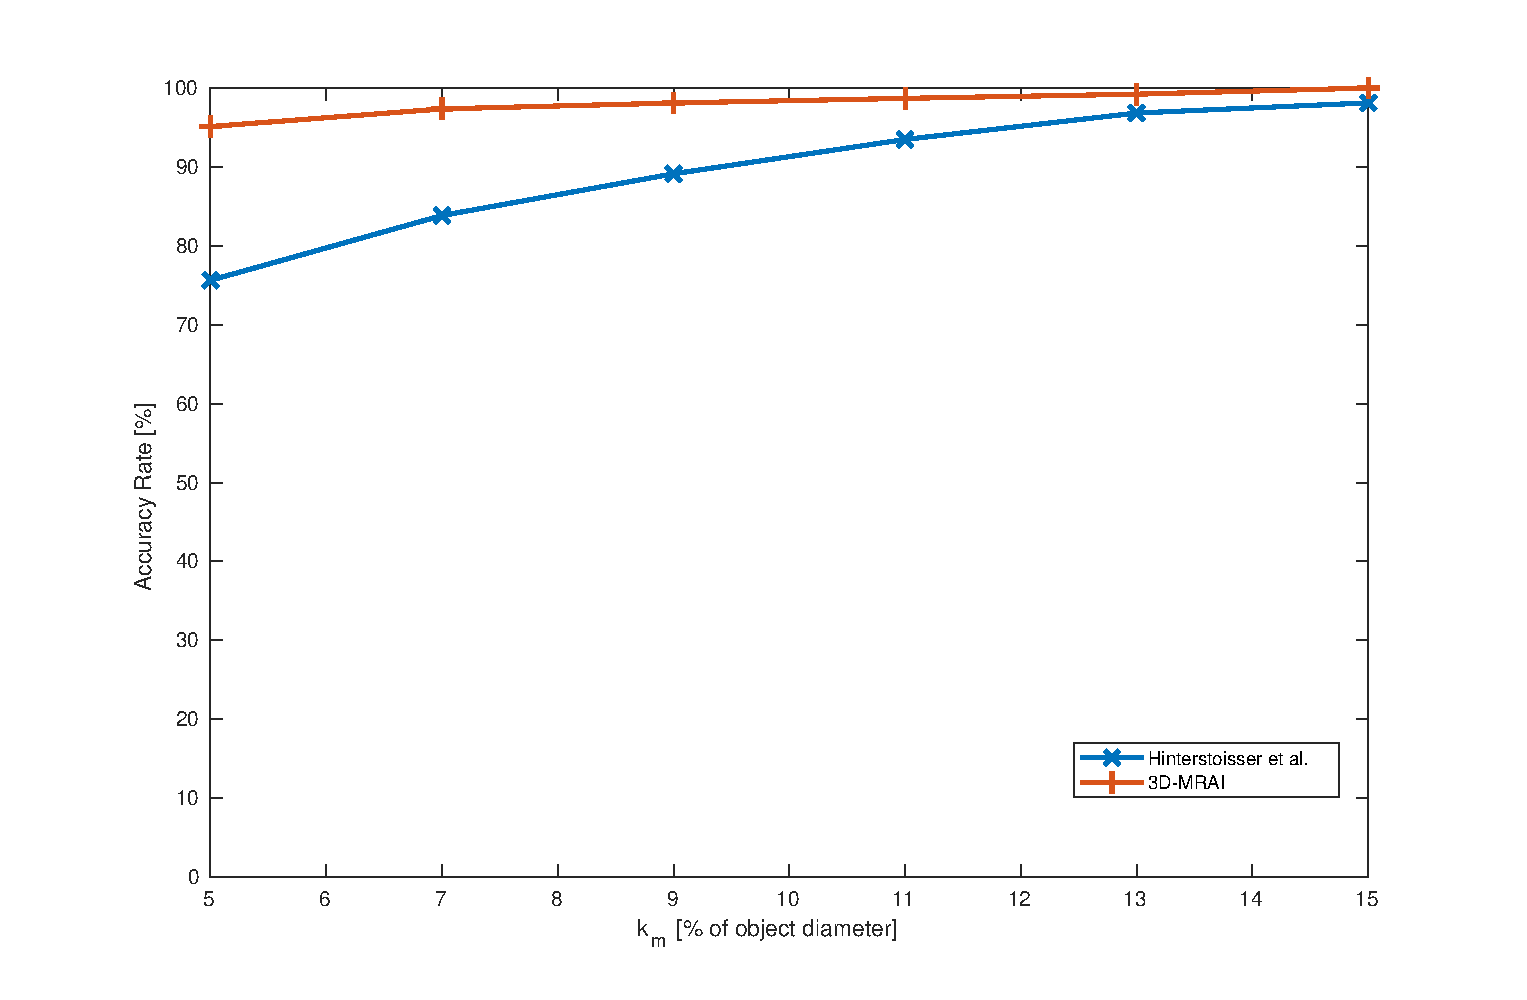
\includegraphics[width=15cm]{accuracy}
  \caption{3D-MRAI和Hinterstorisser等人的算法准确率曲线}
  \label{fig:mrai}
\end{figure}

为了进一步观察算法给出位姿的精度,取$k_m=9\%$时3D-MRAI准确检测的例子,将目标物体的位姿转换为$X,Y,Z,r,p,y$六个直观的变量三维位置和姿态欧拉角,然后于ground truth相比较,得到算法结果在距离和角度上的误差的频率直方图如图\ref{fig:pose-error}所示。
\begin{figure}[ht]
  \centering
  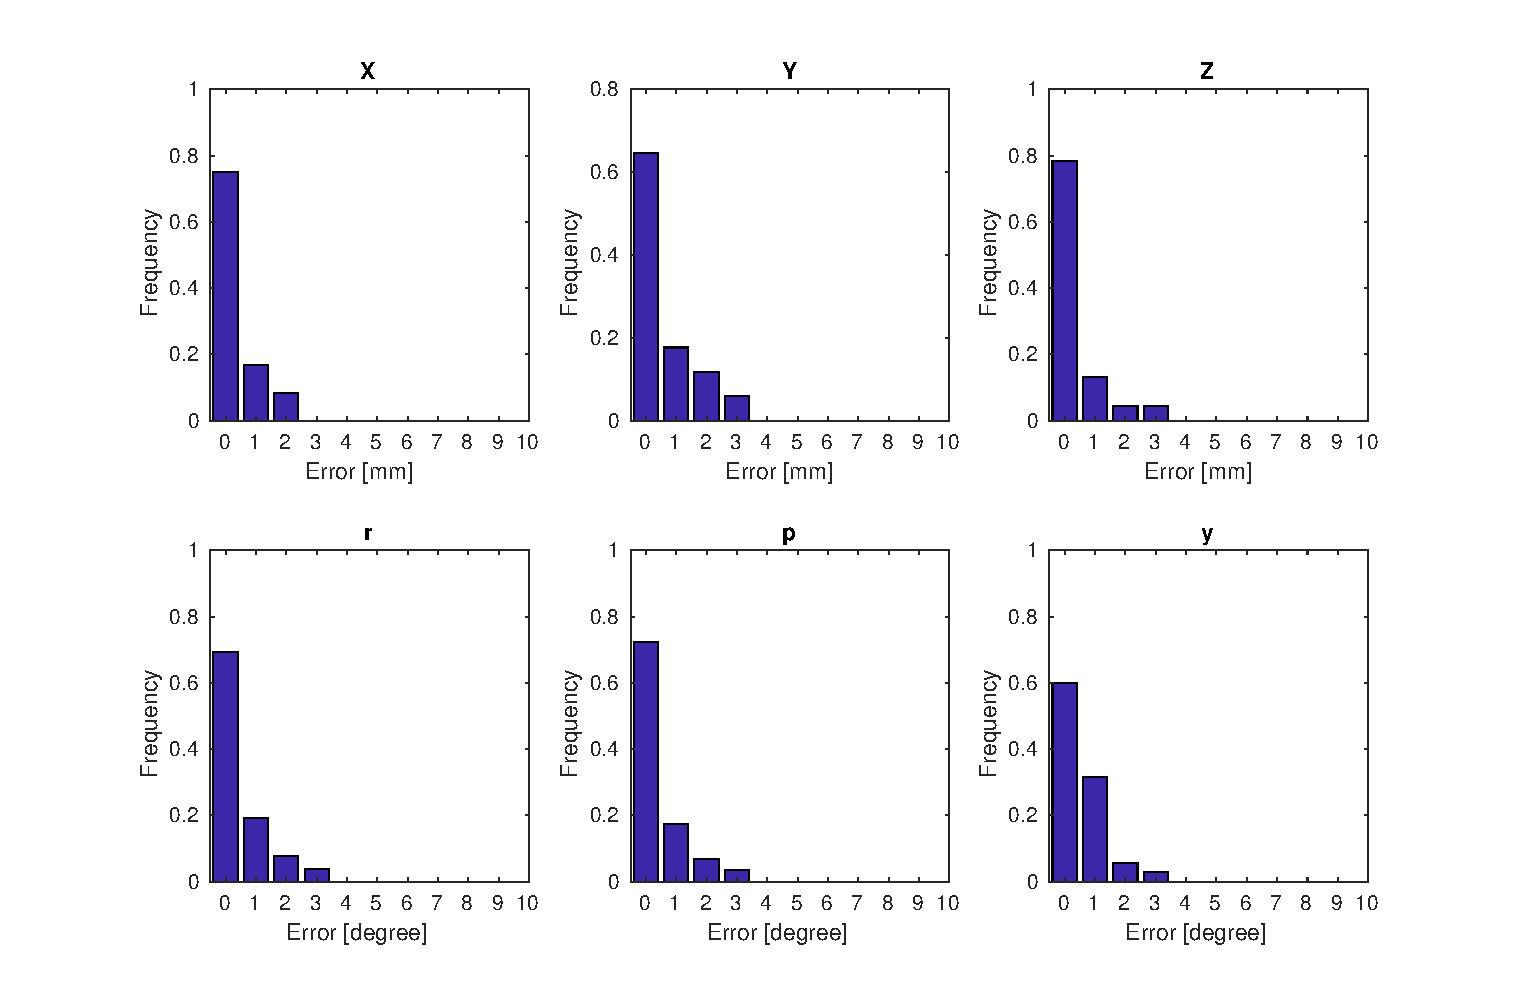
\includegraphics[width=16cm]{pose-error}
  \caption{3D-MRAI算法精度}
  \label{fig:pose-error}
\end{figure}
从图中可以看出3D-MRAI正确检测和估计目标位姿的情况下,在$X,Y,Z$方向下的位置误差大部分分布在$0\sim 1mm$之间,其距离精度在$1mm$左右;在$r,p,y$三个角度下的角度误差也大部分分布在$0\sim 1deg$之间,其角度精度在$1deg$左右。统计图\ref{fig:pose-error}中的数据,可以算出距离误差和角度误差的的均值和方差为:
\begin{equation}
  \begin{array}{ccc}
    e_d &=& 0.82\pm0.21mm\\
    e_a &=& 0.91\pm0.29deg
  \end{array}
\end{equation}

除了关心算法的准确率和精度,算法的运行时间也是我们所关心的。在实验所用的计算机上,本文所设计的3D-MRAI算法与Hinterstorisser等人设计的基于LINEMOD算法的平均帧率如表\ref{tab:mrai-fps}所示。
\begin{table}[ht]
  \centering
  \begin{tabular}{ccc}
    \toprule
    &Hinterstoisser et al.&\bf{3D-MRAI}\\
    \midrule
    FPS&7.6&2.2\\
    \bottomrule
  \end{tabular}
  \caption{3D-MRAI和Hinterstorisser等人的算法准确率}
  \label{tab:mrai-fps}
\end{table}
表中可以看出3D-MRAI的FPS相比Hinterstorisser等人的算法的FPS相对较低,由于使用了深度神经网络相关的算法,涉及到较大的计算量,因此较低的FPS也在情理之中。

综上所述,在$k_m=9\%$时,3D-MRAI算法的准确率为$98.10\%$左右,其估计的位姿的距离精度为$0.82\pm0.21mm$,角度精度为$0.91\pm0.29deg$。

\section{本章小结}
本章介绍了一种基于RGB-D图像的3D目标检测和位姿估计算法3D-MRAI,3D-MARI通过结合3D Faster/Mask R-CNN和A4PCS-ICP算法实现对目标位姿的估计。并通过实验与Hinterstorisser等人的算法比较,得出3D-MRAI算法具有更高的检测准确率,并且位姿精度也更高,但在时间性能上略逊于Hinterstorisser等人的算法。

%%% Local Variables:
%%% mode: latex
%%% TeX-master: "../thesis"
%%% End:
